\begin{titlepage}
  \sffamily
  \vspace*{1.2cm}
  {\color{accent}\rule{2.4cm}{3pt}}\par
  \vspace{1.1cm}
  {\fontsize{46}{50}\selectfont\bfseries\reporttitle\par}
  \vspace{0.5cm}
  {\LARGE\color{ink!85}\reportsubtitle\par}
  \vspace{1.3cm}
  {\large\color{muted}Project report --- Object-oriented programming in Java\par}

  \vfill
  \begin{center}
    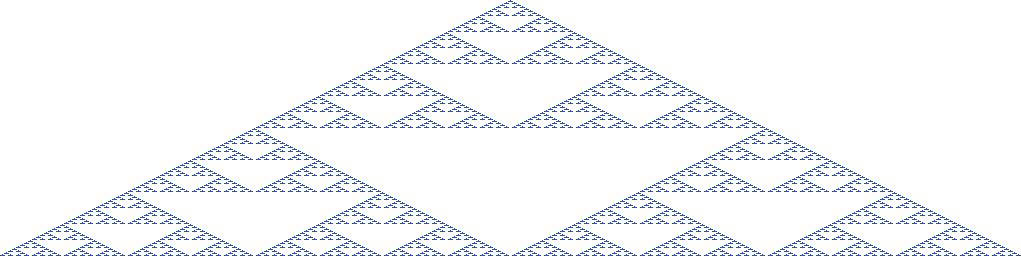
\includegraphics[width=\textwidth]{radius2-fractal}\\[0.5em]
    {\footnotesize\color{muted}The picture drawn by one of the radius-2 rules found by the program
    (\cref{sec:bonus}).}
  \end{center}
  \vfill

  {\large
  \begin{tabular}{@{}>{\color{muted}}l@{\hspace{1.2em}}l@{}}
    Author & \reportauthor \\
    School & Sup Galil\'ee, Universit\'e Sorbonne Paris Nord \\
    Course & Programmation orient\'ee objet (Java), INFO~1, 2023--2024 \\
    Date & \reportdate \\
  \end{tabular}}
  \vspace{0.6cm}
\end{titlepage}
